\documentclass[11pt]{article}
\usepackage[margin=1in]{geometry}
\usepackage{amsmath,amsthm,amssymb}
\usepackage{tikz}
\usetikzlibrary{decorations.pathreplacing,calc,arrows.meta,positioning}

\newtheorem{definition}{Definition}
\newtheorem{lemma}{Lemma}
\newtheorem{corollary}[lemma]{Corollary}
\newtheorem{theorem}[lemma]{Theorem}
\newtheorem{proposition}[lemma]{Proposition}
\newtheorem*{remark}{Remark}

\title{NP-Hardness of the Ordering Recovery Problem}
\date{}

\begin{document}
\maketitle

\section{Preliminaries}

We write $S_N$ for the symmetric group on $\{1, \ldots, N\}$, i.e.\ the set of all $N!$ permutations of $\{1, \ldots, N\}$.

\begin{definition}[Minimum Feedback Arc Set in Tournaments --- FAST]
A tournament $T = (V, A)$ on $N$ vertices is a complete directed graph in which every unordered pair $\{u, v\} \subseteq V$ has exactly one arc: either $(u, v) \in A$ or $(v, u) \in A$. For a linear ordering $\pi$ of $V$, define
\begin{equation}
\mathrm{fas}(T, \pi) = \bigl|\{(u, v) \in A : \pi(u) > \pi(v)\}\bigr|,
\end{equation}
the number of arcs that are ``backwards'' under $\pi$. The FAST decision problem asks: given $T$ and a non-negative integer $k$, does there exist a linear ordering $\pi$ with $\mathrm{fas}(T, \pi) \le k$? This problem is NP-complete \cite{alon2006,charbit2007}.
\end{definition}

\begin{definition}[Ordering Recovery Problem --- ORP]
There are $N$ events $e_1, \ldots, e_N$ assigned to equally spaced time slots by a permutation $\sigma$ drawn uniformly at random from $S_N$: event $e_i$ occupies slot $\sigma(i)$, giving it true timestamp $t_i^* = \sigma(i) \cdot \Delta$ for a fixed spacing $\Delta > 0$. Each event is observed with additive noise:
\begin{equation}
\hat{t}_i = t_i^* + \eta_i, \qquad \eta_i \sim F_i,
\end{equation}
where the $\{\eta_i\}$ are mutually independent and independent of $\sigma$. Throughout, the index $i$ in $\sigma(i)$, $\hat{t}_i$, and $\hat{\pi}(i)$ refers to event $e_i$: $\sigma(i)$ is the true slot of $e_i$, $\hat{t}_i$ is its noisy observation, and $\hat{\pi}(i)$ is the position assigned to $e_i$ by the algorithm.

The ORP decision problem asks: given the observations $\{\hat{t}_i\}$, the distributions $\{F_i\}$, the spacing $\Delta$, and a non-negative rational threshold $K$, does there exist a permutation $\hat{\pi} \in S_N$ with
\begin{equation}
\mathbb{E}\bigl[d_{\mathrm{KT}}(\hat{\pi}, \sigma) \mid \hat{t}\bigr] \le K,
\end{equation}
where
\begin{equation}
\mathbb{E}\bigl[d_{\mathrm{KT}}(\hat{\pi}, \sigma) \mid \hat{t}\bigr] = \mathbb{E}\Bigl[\bigl|\{(i, j) : \sigma(i) < \sigma(j) \text{ and } \hat{\pi}(i) > \hat{\pi}(j)\}\bigr| \;\Big|\; \hat{t}\Bigr]
\end{equation}
is the expected Kendall tau distance between $\hat{\pi}$ and $\sigma$, conditioned on the observed data $\hat{t}$?\footnote{The Kendall tau distance counts the number of unordered pairs $\{i, j\}$ on which two permutations disagree about relative order. We sum over pairs with $i < j$ (rather than all $i \ne j$) to count each unordered pair exactly once; summing over all $i \ne j$ would double-count every pair. For each pair with $i < j$, the formula checks both possible directions of disagreement (either $\sigma$ says $i$ first but $\hat{\pi}$ says $j$ first, or vice versa), and exactly one of these can hold for any discordant pair.}
\end{definition}

\section{Pairwise Decomposition}

Since the Kendall tau distance is a sum over pairs, the conditional expectation decomposes.

\begin{lemma}
For any prior on $\sigma \in S_N$,
\begin{equation}
\mathbb{E}\bigl[d_{\mathrm{KT}}(\hat{\pi}, \sigma) \mid \hat{t}\bigr] = \sum_{i < j} P(\sigma(i) < \sigma(j) \mid \hat{t}) \cdot \mathbf{1}[\hat{\pi}(i) > \hat{\pi}(j)] + P(\sigma(i) > \sigma(j) \mid \hat{t}) \cdot \mathbf{1}[\hat{\pi}(i) < \hat{\pi}(j)].
\end{equation}
\end{lemma}

\begin{proof}
For each pair $(i, j)$ with $i < j$, define the indicator random variable
\begin{equation}
X_{ij}(\sigma, \hat{\pi}) = \mathbf{1}\bigl[\sigma(i) < \sigma(j) \text{ and } \hat{\pi}(i) > \hat{\pi}(j)\bigr] + \mathbf{1}\bigl[\sigma(i) > \sigma(j) \text{ and } \hat{\pi}(i) < \hat{\pi}(j)\bigr].
\end{equation}
This equals~1 precisely when $\sigma$ and $\hat{\pi}$ disagree on the relative order of $i$ and $j$, and equals~0 otherwise. (Exactly one of $\sigma(i) < \sigma(j)$ or $\sigma(i) > \sigma(j)$ holds since $\sigma$ is a permutation, and likewise for $\hat{\pi}$; the pair is discordant when the two orderings differ.) The Kendall tau distance is the total number of discordant pairs:
\begin{equation}
d_{\mathrm{KT}}(\hat{\pi}, \sigma) = \sum_{i < j} X_{ij}(\sigma, \hat{\pi}).
\end{equation}
Taking the conditional expectation given $\hat{t}$ and using linearity:
\begin{equation}
\mathbb{E}\bigl[d_{\mathrm{KT}}(\hat{\pi}, \sigma) \mid \hat{t}\bigr] = \sum_{i < j} \mathbb{E}\bigl[X_{ij}(\sigma, \hat{\pi}) \mid \hat{t}\bigr].
\end{equation}
Since $\hat{\pi}$ is a fixed (non-random) permutation chosen by the algorithm, the indicators $\mathbf{1}[\hat{\pi}(i) > \hat{\pi}(j)]$ and $\mathbf{1}[\hat{\pi}(i) < \hat{\pi}(j)]$ are deterministic constants. Therefore:
\begin{align}
\mathbb{E}\bigl[X_{ij}(\sigma, \hat{\pi}) \mid \hat{t}\bigr]
&= P(\sigma(i) < \sigma(j) \mid \hat{t}) \cdot \mathbf{1}[\hat{\pi}(i) > \hat{\pi}(j)] \notag \\
&\quad + P(\sigma(i) > \sigma(j) \mid \hat{t}) \cdot \mathbf{1}[\hat{\pi}(i) < \hat{\pi}(j)].
\end{align}
Summing over all $\binom{N}{2}$ pairs $i < j$ gives the result.
\end{proof}

\begin{lemma}
Let $p_{ij} = P(\sigma(i) < \sigma(j) \mid \hat{t})$ for $i < j$. This is the posterior probability, given the observed data, that event $i$ truly precedes event $j$. Define the \textbf{most-likely ordering} of the pair $(i, j)$ to be the relative ordering that is more probable under the posterior: ``$i$ before $j$'' if $p_{ij} \ge 1/2$ (i.e.\ the data favours $i$ preceding $j$), and ``$j$ before $i$'' if $p_{ij} < 1/2$ (i.e.\ the data favours $j$ preceding $i$). We say that a permutation $\hat{\pi}$ \textbf{agrees with the most-likely ordering} on $(i,j)$ if $\hat{\pi}$ orders $i$ and $j$ according to the most-likely ordering, and \textbf{disagrees} otherwise. Then
\begin{multline}
\mathbb{E}\bigl[d_{\mathrm{KT}}(\hat{\pi}, \sigma) \mid \hat{t}\bigr] = \sum_{i < j} |2p_{ij} - 1| \cdot \mathbf{1}[\hat{\pi} \text{ disagrees with most-likely ordering on } (i, j)] \\
+\; \sum_{i<j} \min(p_{ij},\, 1 - p_{ij}).
\end{multline}
\end{lemma}

\begin{proof}
By Lemma~1, the contribution of the pair $(i, j)$ with $i < j$ to $\mathbb{E}[d_{\mathrm{KT}}(\hat{\pi}, \sigma) \mid \hat{t}]$ is
\begin{equation}
\ell_{ij}(\hat{\pi}) \;=\; p_{ij} \cdot \mathbf{1}[\hat{\pi}(i) > \hat{\pi}(j)] \;+\; (1 - p_{ij}) \cdot \mathbf{1}[\hat{\pi}(i) < \hat{\pi}(j)],
\end{equation}
where we used $P(\sigma(i) > \sigma(j) \mid \hat{t}) = 1 - P(\sigma(i) < \sigma(j) \mid \hat{t}) = 1 - p_{ij}$, since exactly one of $\sigma(i) < \sigma(j)$ or $\sigma(i) > \sigma(j)$ holds.

Since $\hat{\pi}$ is a permutation, exactly one of $\hat{\pi}(i) < \hat{\pi}(j)$ or $\hat{\pi}(i) > \hat{\pi}(j)$ holds, so exactly one of the two indicators equals~1. We verify all four cases:
\begin{itemize}
\item \emph{Case 1: $p_{ij} \ge 1/2$ and $\hat{\pi}$ agrees} (i.e.\ $\hat{\pi}$ places $i$ before $j$). Then $\mathbf{1}[\hat{\pi}(i) > \hat{\pi}(j)] = 0$ and $\mathbf{1}[\hat{\pi}(i) < \hat{\pi}(j)] = 1$, so $\ell_{ij}(\hat{\pi}) = 1 - p_{ij}$. Since $p_{ij} \ge 1/2$, we have $1 - p_{ij} \le 1/2 \le p_{ij}$, so $\ell_{ij}(\hat{\pi}) = \min(p_{ij},\, 1 - p_{ij})$.

\item \emph{Case 2: $p_{ij} \ge 1/2$ and $\hat{\pi}$ disagrees} (i.e.\ $\hat{\pi}$ places $j$ before $i$). Then $\mathbf{1}[\hat{\pi}(i) > \hat{\pi}(j)] = 1$ and $\mathbf{1}[\hat{\pi}(i) < \hat{\pi}(j)] = 0$, so $\ell_{ij}(\hat{\pi}) = p_{ij}$. Since $p_{ij} \ge 1/2$, we have $p_{ij} = \max(p_{ij},\, 1 - p_{ij})$.

\item \emph{Case 3: $p_{ij} < 1/2$ and $\hat{\pi}$ agrees} (i.e.\ $\hat{\pi}$ places $j$ before $i$). Then $\mathbf{1}[\hat{\pi}(i) > \hat{\pi}(j)] = 1$ and $\mathbf{1}[\hat{\pi}(i) < \hat{\pi}(j)] = 0$, so $\ell_{ij}(\hat{\pi}) = p_{ij}$. Since $p_{ij} < 1/2$, we have $p_{ij} = \min(p_{ij},\, 1 - p_{ij})$.

\item \emph{Case 4: $p_{ij} < 1/2$ and $\hat{\pi}$ disagrees} (i.e.\ $\hat{\pi}$ places $i$ before $j$). Then $\mathbf{1}[\hat{\pi}(i) > \hat{\pi}(j)] = 0$ and $\mathbf{1}[\hat{\pi}(i) < \hat{\pi}(j)] = 1$, so $\ell_{ij}(\hat{\pi}) = 1 - p_{ij}$. Since $p_{ij} < 1/2$, we have $1 - p_{ij} > 1/2 > p_{ij}$, so $\ell_{ij}(\hat{\pi}) = \max(p_{ij},\, 1 - p_{ij})$.
\end{itemize}

In all four cases: if $\hat{\pi}$ agrees with the most-likely ordering, then $\ell_{ij}(\hat{\pi}) = \min(p_{ij},\, 1 - p_{ij})$; if it disagrees, then $\ell_{ij}(\hat{\pi}) = \max(p_{ij},\, 1 - p_{ij})$. Now observe that
\begin{equation}
\max(p,\, 1-p) = \min(p,\, 1-p) + |2p - 1|
\end{equation}
for all $p \in [0,1]$ (since $\max(p, 1-p) - \min(p, 1-p) = |p - (1-p)| = |2p - 1|$). Therefore:
\begin{equation}
\ell_{ij}(\hat{\pi}) = |2p_{ij} - 1| \cdot \mathbf{1}[\hat{\pi} \text{ disagrees with most-likely ordering on } (i,j)] \;+\; \min(p_{ij},\, 1 - p_{ij}).
\end{equation}
Summing over all pairs $i < j$:
\begin{multline}
\mathbb{E}\bigl[d_{\mathrm{KT}}(\hat{\pi}, \sigma) \mid \hat{t}\bigr] = \sum_{i<j} \ell_{ij}(\hat{\pi}) \\
= \sum_{i < j} |2p_{ij} - 1| \cdot \mathbf{1}[\hat{\pi} \text{ disagrees with most-likely ordering on } (i, j)] + \sum_{i<j} \min(p_{ij},\, 1 - p_{ij}). \qedhere
\end{multline}
\end{proof}

\section{The Reduction}

\begin{theorem}
The Ordering Recovery Problem (Definition~2) is NP-hard.
\end{theorem}

\begin{proof}
We reduce FAST to ORP in polynomial time. Let $T = (V, A)$ be a tournament on $N$ vertices $V = \{1, \ldots, N\}$, and let $k$ be a non-negative integer. Set $M = \binom{N}{2}$ and fix an enumeration of the unordered pairs of vertices as $\{i_1, j_1\}, \ldots, \{i_M, j_M\}$ with $i_r < j_r$.
The following table summarises how each component of the FAST decision instance maps to a component of the ORP decision instance, with references to the subsections where each part is established.

\begin{center}
\renewcommand{\arraystretch}{1.3}
\begin{tabular}{@{}p{0.38\textwidth}@{\;$\longrightarrow$\;}p{0.44\textwidth}@{\quad}p{0.06\textwidth}@{}}
\hline
\textbf{FAST instance $(T, k)$} & \textbf{ORP instance $f(T, k)$} & \textbf{Ref.} \\
\hline
$N$ tournament vertices & (used only to define the $M$ pairs below) & \\
$M = \binom{N}{2}$ vertex pairs $\{i_r, j_r\}$ & $M$ blocks, each containing two events $e_r^{(1)}, e_r^{(2)}$ in adjacent time slots $\{2r{-}1, 2r\}$; total $2M$ events with $\Delta = 1$ & \S\ref{step:construction} \\
Arc direction: $(i_r, j_r) \in A$ or $(j_r, i_r) \in A$ & Noise distributions $F_r^{(1)}, F_r^{(2)}$ chosen so the most-likely ordering matches the arc direction, with $|2p_r - 1| = 1/2$, where $p_r = P(e_r^{(1)} \text{ truly precedes } e_r^{(2)} \mid \hat{t})$ is the posterior probability for intra-block pair $r$ & \S\ref{step:construction}, \S\ref{step:posteriors} \\
Threshold $k$ & Threshold $K = k/2 + M/4$ & \S\ref{step:reduction} \\
\hline
\end{tabular}
\end{center}
The detailed construction of $f$ and verification of correctness follow in \S\ref{step:construction}--\S\ref{step:reduction}.
\end{proof}

\subsection{Construction}\label{step:construction}

Define an ORP instance with $2M$ events and spacing $\Delta = 1$. For each pair $r = 1, \ldots, M$, introduce two events $e_r^{(1)}$ and $e_r^{(2)}$ occupying time slots $\{2r-1, 2r\}$ (called \emph{block $r$}), with observed timestamps $\hat{t}_r^{(1)} = 2r - 1$ and $\hat{t}_r^{(2)} = 2r$. Their noise distributions depend on the arc direction in $T$:

\begin{itemize}
\item If $(i_r, j_r) \in A$\;\;(%
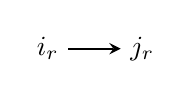
\begin{tikzpicture}[baseline=-0.5ex]
\node (i) at (0,0) {$i_r$};
\node (j) at (1.2,0) {$j_r$};
\draw[->,>=stealth,thick] (i) -- (j);
\end{tikzpicture}):
\begin{equation}
F_r^{(1)}(k) = \begin{cases} 3/4 & \text{if } k = 0, \\ 1/4 & \text{if } k = -1, \\ 0 & \text{otherwise,} \end{cases}
\qquad
F_r^{(2)}(k) = \begin{cases} 1/2 & \text{if } k = 0, \\ 1/2 & \text{if } k = 1, \\ 0 & \text{otherwise.} \end{cases}
\end{equation}

\item If $(j_r, i_r) \in A$\;\;(%
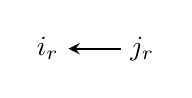
\begin{tikzpicture}[baseline=-0.5ex]
\node (i) at (0,0) {$i_r$};
\node (j) at (1.2,0) {$j_r$};
\draw[<-,>=stealth,thick] (i) -- (j);
\end{tikzpicture}):
\begin{equation}
F_r^{(1)}(k) = \begin{cases} 1/4 & \text{if } k = 0, \\ 3/4 & \text{if } k = -1, \\ 0 & \text{otherwise,} \end{cases}
\qquad
F_r^{(2)}(k) = \begin{cases} 1/2 & \text{if } k = 0, \\ 1/2 & \text{if } k = 1, \\ 0 & \text{otherwise.} \end{cases}
\end{equation}
\end{itemize}

\noindent\emph{Design rationale.} The noise distributions are engineered to achieve two properties. First, the finite support of each noise distribution confines each event to its own block: because $F_r^{(1)}$ has support $\{0, -1\}$ and $F_r^{(2)}$ has support $\{0, 1\}$, the only slots compatible with the observed timestamps are the two slots within block $r$ (this is verified in \S\ref{step:blocks}). Note that this confinement is a property of the \emph{true} timestamps --- the observed timestamps $\hat{t}_r^{(1)} = 2r-1$ and $\hat{t}_r^{(2)} = 2r$ are fixed by construction and always fall within the block by definition, but the key point is that the noise support forces the true timestamps to also stay within the block.

Second, the asymmetry between the two arc-direction cases (swapping $3/4$ and $1/4$ in $F_r^{(1)}$) ensures that the posterior probability $p_r$ equals $3/4$ or $1/4$ depending on the arc direction, so that the most-likely ordering always matches the arc direction and the quantity $|2p_r - 1|$ --- which is the per-pair weight in the cost formula of Lemma~2 --- equals $1/2$ uniformly across all $M$ pairs (as computed in \S\ref{step:posteriors}). The specific values $3/4$ and $1/4$ are not essential; any values $p$ and $1-p$ with $p \ne 1/2$ would work, as long as $|2p - 1|$ is the same for every pair.

\subsection{Block structure and inter-block independence}\label{step:blocks}

By Lemma~2, the expected Kendall tau distance is a sum over all $\binom{2M}{2}$ event pairs of per-pair contributions $\ell_{ij}(\hat{\pi})$. Recall that by construction, the $2M$ time slots partition into $M$ disjoint blocks, where block $r$ consists of slots $\{2r-1, 2r\}$.

Although $\sigma$ is drawn uniformly from $S_{2M}$, the observed data $\hat{t}$ together with the finite support of the noise distributions restrict which permutations have nonzero posterior probability. We verify this for each event:

\begin{itemize}
\item \emph{Event $e_r^{(1)}$}: Its observed timestamp is $\hat{t}_r^{(1)} = 2r - 1$. If $\sigma$ assigns $e_r^{(1)}$ to slot $s$, then its true timestamp is $t^* = s$ (since $\Delta = 1$) and the required noise realisation is $\eta = \hat{t}_r^{(1)} - t^* = (2r - 1) - s$. The distribution $F_r^{(1)}$ has support $\{0, -1\}$ (in both arc-direction cases), so we need $(2r - 1) - s \in \{0, -1\}$, i.e.\ $s = 2r - 1$ or $s = 2r$. These are exactly the two slots of block $r$.

\item \emph{Event $e_r^{(2)}$}: Its observed timestamp is $\hat{t}_r^{(2)} = 2r$. If $\sigma$ assigns $e_r^{(2)}$ to slot $s$, the required noise is $\eta = \hat{t}_r^{(2)} - t^* = 2r - s$. The distribution $F_r^{(2)}$ has support $\{0, 1\}$ (in both arc-direction cases), so we need $2r - s \in \{0, 1\}$, i.e.\ $s = 2r$ or $s = 2r - 1$. Again, exactly the two slots of block $r$.
\end{itemize}

Since both events in block $r$ must occupy the two slots of block $r$, and events from different blocks are similarly confined to their own blocks, the posterior on $\sigma$ reduces to $M$ independent binary choices: for each block $r$, either $e_r^{(1)}$ occupies slot $2r - 1$ and $e_r^{(2)}$ occupies slot $2r$, or vice versa.

Event pairs fall into two types:

\begin{itemize}
\item \emph{Inter-block pair} (events from distinct blocks $r \ne s$): Assume $r < s$ without loss of generality. The largest slot in block $r$ is $2r$, and the smallest slot in block $s$ is $2s - 1 \ge 2(r+1) - 1 = 2r + 1 > 2r$. So every slot in block $r$ is strictly less than every slot in block $s$. Since each event is confined to the two slots of its own block (as shown above), any event in block $r$ always occupies a smaller slot than any event in block $s$, regardless of which binary choice is made within each block. Thus $p_{ab} = 1$ when event $a$ is in the earlier block and event $b$ is in the later block. By Lemma~2, the per-pair contribution is $\ell_{ab}(\hat{\pi}) = |2 \cdot 1 - 1| \cdot \mathbf{1}[\text{disagree}] + \min(1, 0) = \mathbf{1}[\text{disagree}]$. This contribution is zero if $\hat{\pi}$ places $a$ before $b$ (agreeing with the deterministic ordering), and equals $1$ if $\hat{\pi}$ places $b$ before $a$ (disagreeing). In particular:
\begin{itemize}
\item For any permutation that lists blocks in increasing order (as the lifting construction in \S\ref{step:reduction} does), all inter-block contributions are zero.
\item For an arbitrary permutation $\hat{\pi}$ that may interleave events from different blocks, inter-block contributions are non-negative: $\ell_{ab}(\hat{\pi}) \ge 0$. Any inter-block disagreement can only \emph{increase} the cost relative to a permutation that respects block order.
\end{itemize}

\item \emph{Intra-block pair} (events $e_r^{(1)}$ and $e_r^{(2)}$ from the same block): The relative order depends on the binary choice within block $r$, so $p_r \notin \{0, 1\}$ in general.
\end{itemize}

\begin{figure}[ht]
\centering
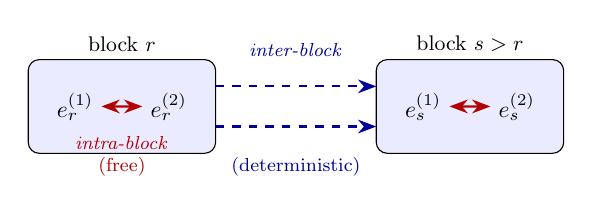
\begin{tikzpicture}[>=Stealth, scale=0.85, every node/.style={scale=0.85}]
  % Block r
  \draw[rounded corners, fill=blue!8] (0,0) rectangle (2.8,1.4);
  \node[anchor=south] at (1.4,1.4) {\small block $r$};
  \node (e1r) at (0.7,0.7) {$e_r^{(1)}$};
  \node (e2r) at (2.1,0.7) {$e_r^{(2)}$};

  % Within-pair arrow
  \draw[<->,thick,red!70!black] (e1r) -- (e2r);
  \node[red!70!black, font=\footnotesize] at (1.4,0.15) {\emph{intra-block}};
  \node[red!70!black, font=\footnotesize] at (1.4,-0.2) {(free)};

  % Block s
  \draw[rounded corners, fill=blue!8] (5.2,0) rectangle (8.0,1.4);
  \node[anchor=south] at (6.6,1.4) {\small block $s > r$};
  \node (e1s) at (5.9,0.7) {$e_s^{(1)}$};
  \node (e2s) at (7.3,0.7) {$e_s^{(2)}$};

  % Within-pair arrow
  \draw[<->,thick,red!70!black] (e1s) -- (e2s);

  % Cross-pair arrows
  \draw[->,thick,blue!60!black,dashed] (2.8,1.0) -- (5.2,1.0);
  \draw[->,thick,blue!60!black,dashed] (2.8,0.4) -- (5.2,0.4);
  \node[blue!60!black, font=\footnotesize, align=center] at (4.0,1.55) {\emph{inter-block}};
  \node[blue!60!black, font=\footnotesize, align=center] at (4.0,-0.2) {(deterministic)};
\end{tikzpicture}
\caption{Inter-block orderings are deterministic (all slots in block $r$ are less than all slots in block $s$ when $r < s$). Intra-block orderings within each block are the only free variables.}
\label{fig:interblock}
\end{figure}

Since there are $2M$ events in total, the number of event pairs is $\binom{2M}{2} = M(2M - 1)$. Each of the $M$ blocks contributes exactly one intra-block pair (its two events), giving $M$ intra-block pairs. The remaining $\binom{2M}{2} - M = 2M(M-1)$ pairs are inter-block pairs. Inter-block contributions are non-negative and are zero for any permutation that respects block order (as shown above). Consequently, any permutation that minimises the expected Kendall tau distance can be assumed to respect block order without loss of generality (since violating it can only increase the cost). For such permutations, the expected Kendall tau distance depends only on the $M$ intra-block decisions: for each block $r$, choose which of $e_r^{(1)}$ and $e_r^{(2)}$ to place first. These decisions are independent because different blocks do not interact --- each event is confined to its own block's two slots.

\subsection{Pairwise posteriors}\label{step:posteriors}

By \S\ref{step:blocks}, for any permutation that respects block order, the expected Kendall tau distance depends only on the $M$ intra-block decisions (since inter-block contributions are zero for such permutations). By Lemma~2, the contribution of intra-block pair $r$ is
\begin{equation}\label{eq:per-pair}
\ell_r(\hat{\pi}) = |2p_r - 1| \cdot \mathbf{1}[\hat{\pi} \text{ disagrees with most-likely ordering on pair } r] + \min(p_r, 1 - p_r),
\end{equation}
where $p_r = P(e_r^{(1)} \text{ truly precedes } e_r^{(2)} \mid \hat{t})$. The first term depends on $\hat{\pi}$'s choice for pair $r$; the second does not. To evaluate this, we need to compute $p_r$ for each block.

For every pair $r$, $\hat{t}_r^{(1)} = 2r - 1$ and $\hat{t}_r^{(2)} = 2r$. Let $\sigma_r$ denote the binary choice within block $r$. The two cases determine the noise realisations via $\eta_r^{(a)} = \hat{t}_r^{(a)} - t_r^{*(a)}$:
\begin{align}
e_r^{(1)} \to \text{slot } 2r\!-\!1,\; e_r^{(2)} \to \text{slot } 2r &: \quad t_r^{*(1)} = 2r-1,\; t_r^{*(2)} = 2r, \quad \text{so } \eta_r^{(1)} = 0,\; \eta_r^{(2)} = 0. \\
e_r^{(1)} \to \text{slot } 2r,\; e_r^{(2)} \to \text{slot } 2r\!-\!1 &: \quad t_r^{*(1)} = 2r,\; t_r^{*(2)} = 2r-1, \quad \text{so } \eta_r^{(1)} = -1,\; \eta_r^{(2)} = 1.
\end{align}

Under a uniform prior on $\sigma_r$ (each case has prior probability $1/2$), Bayes' rule gives the posterior probability of the first case. Let $D = \hat{t}$ denote the observed data. The likelihood of $D$ under each case is the product of the noise probabilities (since the noise variables are independent given $\sigma_r$):
\begin{align}
P(D \mid \text{case 1}) &= F_r^{(1)}(0) \cdot F_r^{(2)}(0), \\
P(D \mid \text{case 2}) &= F_r^{(1)}(-1) \cdot F_r^{(2)}(1).
\end{align}
By Bayes' rule:
\begin{equation}
p_r = P(\text{case 1} \mid D) = \frac{P(D \mid \text{case 1}) \cdot P(\text{case 1})}{P(D \mid \text{case 1}) \cdot P(\text{case 1}) + P(D \mid \text{case 2}) \cdot P(\text{case 2})}.
\end{equation}
Since $P(\text{case 1}) = P(\text{case 2}) = 1/2$, the prior factors cancel:
\begin{equation}
p_r = \frac{F_r^{(1)}(0) \cdot F_r^{(2)}(0)}{F_r^{(1)}(0) \cdot F_r^{(2)}(0) + F_r^{(1)}(-1) \cdot F_r^{(2)}(1)}.
\end{equation}

We now substitute the noise distributions from \S\ref{step:construction} for each arc direction:

\begin{itemize}
\item When $(i_r, j_r) \in A$: $F_r^{(1)}(0) = 3/4$, $F_r^{(1)}(-1) = 1/4$, $F_r^{(2)}(0) = 1/2$, $F_r^{(2)}(1) = 1/2$. So:
\begin{equation}
p_r = \frac{(3/4)(1/2)}{(3/4)(1/2) + (1/4)(1/2)} = \frac{3/8}{3/8 + 1/8} = \frac{3/8}{4/8} = \frac{3}{4}.
\end{equation}
Since $p_r = 3/4 > 1/2$, the most-likely ordering is ``$e_r^{(1)}$ before $e_r^{(2)}$'', which corresponds to the arc direction $(i_r, j_r)$. Substituting into (\ref{eq:per-pair}): $|2 \cdot 3/4 - 1| = 1/2$ and $\min(3/4, 1/4) = 1/4$.

\item When $(j_r, i_r) \in A$: $F_r^{(1)}(0) = 1/4$, $F_r^{(1)}(-1) = 3/4$, $F_r^{(2)}(0) = 1/2$, $F_r^{(2)}(1) = 1/2$. So:
\begin{equation}
p_r = \frac{(1/4)(1/2)}{(1/4)(1/2) + (3/4)(1/2)} = \frac{1/8}{1/8 + 3/8} = \frac{1/8}{4/8} = \frac{1}{4}.
\end{equation}
Since $p_r = 1/4 < 1/2$, the most-likely ordering is ``$e_r^{(2)}$ before $e_r^{(1)}$'', which again corresponds to the arc direction $(j_r, i_r)$. Substituting into (\ref{eq:per-pair}): $|2 \cdot 1/4 - 1| = 1/2$ and $\min(1/4, 3/4) = 1/4$.
\end{itemize}

\noindent\textbf{Summary.} In both arc-direction cases:
\begin{enumerate}
\item The most-likely ordering on pair $r$ agrees with the arc direction in $T$.
\item The weight $|2p_r - 1| = 1/2$ for every $r$. (This is the coefficient of the disagreement indicator in Lemma~2's formula, applied to pair $r$.)
\item The constant term $\min(p_r, 1-p_r) = 1/4$ for every $r$. (This is the $\hat{\pi}$-independent part of pair $r$'s contribution in Lemma~2's formula.)
\end{enumerate}

\subsection{Reducing FAST to ORP}\label{step:reduction}

We define a many-one reduction $f$ from FAST to ORP. Given any FAST instance $(T, k)$, the reduction $f$ maps it to the ORP instance constructed in \S\ref{step:construction}--\S\ref{step:posteriors} (with $2M$ events, noise distributions determined by $T$, observed timestamps $\hat{t}_r^{(a)}$, spacing $\Delta = 1$) together with the threshold $K = k/2 + M/4$. We write $f(T, k)$ for this ORP instance. We must show two things: (1) $f$ is computable in polynomial time, and (2) $(T, k) \in \mathrm{FAST} \iff f(T, k) \in \mathrm{ORP}$.

\smallskip
\noindent\textbf{The lifting construction.}
Given a linear ordering $\pi'$ of $V = \{1, \ldots, N\}$, we construct a specific permutation $\hat{\pi}$ of the $2M$ events --- called the \emph{lifting} of $\pi'$ --- as follows. Place the $M$ blocks in the fixed order $1, 2, \ldots, M$. Within block $r$ (corresponding to the vertex pair $\{i_r, j_r\}$), place $e_r^{(1)}$ before $e_r^{(2)}$ if $\pi'(i_r) < \pi'(j_r)$, and $e_r^{(2)}$ before $e_r^{(1)}$ otherwise. This is well-defined because $\pi'$ is a total order on $V$, so for each pair $\{i_r, j_r\}$ exactly one of the two cases holds. The resulting $\hat{\pi}$ is a valid permutation of the $2M$ events (it lists each event exactly once: the $2M$ events are enumerated block by block, with each block contributing its two events in a definite order). Since blocks are listed in order, all inter-block pairs have the earlier-block event placed first, so inter-block disagreements are zero.

\begin{figure}[ht]
\centering
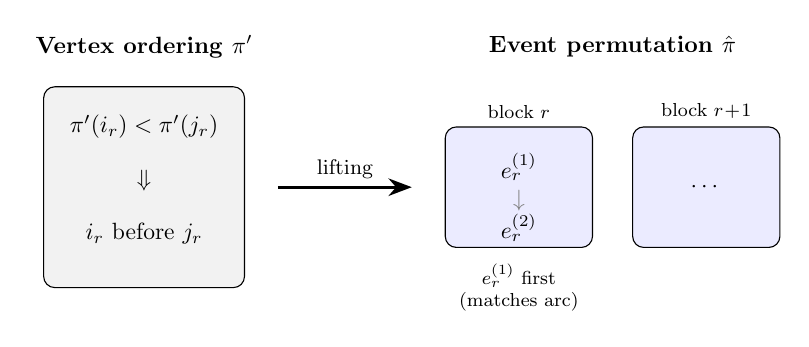
\begin{tikzpicture}[>=Stealth, scale=0.85, every node/.style={scale=0.85}]
  % Left side: vertex ordering
  \node[font=\bfseries] at (1.5,3.8) {Vertex ordering $\pi'$};
  \draw[rounded corners, fill=gray!10] (0,0.2) rectangle (3.0,3.2);
  \node at (1.5,2.6) {$\pi'(i_r) < \pi'(j_r)$};
  \node at (1.5,1.8) {$\Downarrow$};
  \node at (1.5,1.0) {$i_r$ before $j_r$};

  % Arrow
  \draw[->,very thick] (3.5,1.7) -- (5.5,1.7);
  \node[font=\small,above] at (4.5,1.7) {lifting};

  % Right side: event permutation
  \node[font=\bfseries] at (8.5,3.8) {Event permutation $\hat{\pi}$};

  % Block r
  \draw[rounded corners, fill=blue!8] (6.0,0.8) rectangle (8.2,2.6);
  \node[font=\footnotesize,anchor=south] at (7.1,2.6) {block $r$};
  \node at (7.1,2.0) {$e_r^{(1)}$};
  \node[gray] at (7.1,1.5) {$\downarrow$};
  \node at (7.1,1.1) {$e_r^{(2)}$};

  % Block r+1 placeholder
  \draw[rounded corners, fill=blue!8] (8.8,0.8) rectangle (11.0,2.6);
  \node[font=\footnotesize,anchor=south] at (9.9,2.6) {block $r\!+\!1$};
  \node at (9.9,1.7) {$\cdots$};

  % Label
  \node[font=\footnotesize, align=center] at (7.1,0.2) {$e_r^{(1)}$ first\\(matches arc)};
\end{tikzpicture}
\caption{The lifting construction: a vertex ordering $\pi'$ determines the internal order of each block. If $\pi'$ ranks $i_r$ before $j_r$, then $e_r^{(1)}$ is placed before $e_r^{(2)}$ in block $r$, agreeing with the arc direction $(i_r, j_r) \in A$.}
\label{fig:lifting}
\end{figure}

\noindent\emph{Intra-block disagreements equal backward arcs.}
We verify that $\hat{\pi}$ disagrees with the most-likely ordering on pair $r$ if and only if $\pi'$ disagrees with the arc direction on $\{i_r, j_r\}$. By \S\ref{step:posteriors}, the most-likely ordering on pair $r$ is ``$e_r^{(1)}$ before $e_r^{(2)}$'' when $(i_r, j_r) \in A$, and ``$e_r^{(2)}$ before $e_r^{(1)}$'' when $(j_r, i_r) \in A$. Consider the case $(i_r, j_r) \in A$:
\begin{itemize}
\item If $\pi'(i_r) < \pi'(j_r)$ (i.e.\ $\pi'$ agrees with the arc), then the lifting places $e_r^{(1)}$ before $e_r^{(2)}$, which agrees with the most-likely ordering. No disagreement.
\item If $\pi'(i_r) > \pi'(j_r)$ (i.e.\ $\pi'$ disagrees with the arc), then the lifting places $e_r^{(2)}$ before $e_r^{(1)}$, which disagrees with the most-likely ordering. Disagreement.
\end{itemize}
The case $(j_r, i_r) \in A$ is symmetric. Therefore, in both cases, $\hat{\pi}$ disagrees with the most-likely ordering on pair $r$ $\iff$ the arc on $\{i_r, j_r\}$ is backward under $\pi'$. The total number of intra-block disagreements equals $\mathrm{fas}(T, \pi')$.

\smallskip
\noindent\emph{Computing the expected Kendall tau distance.}
By \S\ref{step:blocks}, inter-block contributions are zero. By \S\ref{step:posteriors}, each intra-block pair has weight $|2p_r - 1| = 1/2$ and constant term $\min(p_r, 1-p_r) = 1/4$. Substituting into the formula from Lemma~2 (with the sum restricted to the $M$ intra-block pairs, since inter-block terms vanish):
\begin{align}
\mathbb{E}\bigl[d_{\mathrm{KT}}(\hat{\pi}, \sigma) \mid \hat{t}\bigr]
&= \sum_{r=1}^{M} \Bigl[\frac{1}{2} \cdot \mathbf{1}[\hat{\pi} \text{ disagrees on pair } r] + \frac{1}{4}\Bigr] \notag \\
&= \frac{1}{2} \cdot \mathrm{fas}(T, \pi') + \frac{M}{4}.
\end{align}

\smallskip
\noindent\emph{Any combination of intra-block choices is realisable.}
For any vector of binary choices $(c_1, \ldots, c_M) \in \{0, 1\}^M$ (where $c_r = 0$ means ``$e_r^{(1)}$ first'' and $c_r = 1$ means ``$e_r^{(2)}$ first''), there exists a valid permutation of the $2M$ events that realises these choices: list the blocks in order $1, 2, \ldots, M$, and within block $r$ place the events according to $c_r$. This produces a sequence of $2M$ distinct events (each appears exactly once since the blocks partition the event set), which is a valid permutation.

\smallskip
\noindent\emph{Any permutation can be improved to a lifted permutation.}
Let $\hat{\pi}$ be any permutation of the $2M$ events. For each block $r$, $\hat{\pi}$ induces a definite binary choice (which of $e_r^{(1)}, e_r^{(2)}$ comes first). By the realisability result, there exists a lifted permutation $\hat{\pi}^*$ --- constructed from some vertex ordering $\pi'$ --- that makes the same $M$ intra-block choices as $\hat{\pi}$. The lifted permutation $\hat{\pi}^*$ lists blocks in increasing order, so all its inter-block contributions are zero (by \S\ref{step:blocks}). The original $\hat{\pi}$ may interleave events from different blocks, incurring non-negative inter-block contributions. Since the intra-block contributions are identical (same binary choices) and the inter-block contributions can only be smaller for $\hat{\pi}^*$:
\begin{equation}
\mathbb{E}\bigl[d_{\mathrm{KT}}(\hat{\pi}^*, \sigma) \mid \hat{t}\bigr] \le \mathbb{E}\bigl[d_{\mathrm{KT}}(\hat{\pi}, \sigma) \mid \hat{t}\bigr].
\end{equation}
Moreover, the cost of $\hat{\pi}^*$ is determined entirely by its intra-block choices:
\begin{equation}
\mathbb{E}\bigl[d_{\mathrm{KT}}(\hat{\pi}^*, \sigma) \mid \hat{t}\bigr] = \frac{1}{2} \cdot \mathrm{fas}(T, \pi') + \frac{M}{4}.
\end{equation}

\smallskip
\noindent\textbf{Correctness of the reduction: $(T, k) \in \mathrm{FAST} \iff f(T, k) \in \mathrm{ORP}$.}

\smallskip
\noindent ($\Rightarrow$)\; Suppose $(T, k) \in \mathrm{FAST}$, i.e.\ there exists a linear ordering $\pi'$ of $V$ with $\mathrm{fas}(T, \pi') \le k$. Lift $\pi'$ to a permutation $\hat{\pi}$ of the $2M$ events as described above. Then:
\begin{equation}
\mathbb{E}\bigl[d_{\mathrm{KT}}(\hat{\pi}, \sigma) \mid \hat{t}\bigr] = \frac{1}{2} \cdot \mathrm{fas}(T, \pi') + \frac{M}{4} \le \frac{k}{2} + \frac{M}{4} = K.
\end{equation}
So $\hat{\pi}$ witnesses that $f(T, k) \in \mathrm{ORP}$.

\smallskip
\noindent ($\Leftarrow$)\; Suppose $f(T, k) \in \mathrm{ORP}$, i.e.\ there exists a permutation $\hat{\pi}$ of the $2M$ events with $\mathbb{E}[d_{\mathrm{KT}}(\hat{\pi}, \sigma) \mid \hat{t}] \le K$. By the result above, there exists a vertex ordering $\pi'$ whose lifting $\hat{\pi}^*$ has cost at most that of $\hat{\pi}$. Then:
\begin{equation}
\frac{1}{2} \cdot \mathrm{fas}(T, \pi') + \frac{M}{4} = \mathbb{E}\bigl[d_{\mathrm{KT}}(\hat{\pi}^*, \sigma) \mid \hat{t}\bigr] \le \mathbb{E}\bigl[d_{\mathrm{KT}}(\hat{\pi}, \sigma) \mid \hat{t}\bigr] \le K = \frac{k}{2} + \frac{M}{4}.
\end{equation}
Subtracting $M/4$ and multiplying by $2$: $\mathrm{fas}(T, \pi') \le k$. So $(T, k) \in \mathrm{FAST}$.

\smallskip
\noindent\textbf{Polynomial time.} The ORP instance $f(T, k)$ has $2M = N(N-1)$ events, each with a noise distribution specified by $O(1)$ rational parameters, observed timestamps in $\{1, \ldots, 2M\}$, and a rational threshold $K = k/2 + M/4$. All of these are computable in time polynomial in $N$ and $\log k$, so $f$ is a polynomial-time computable function.

\smallskip
\noindent\textbf{Conclusion.} The function $f$ is a polynomial-time many-one reduction from FAST to ORP: $f$ is computable in polynomial time, and $(T, k) \in \mathrm{FAST} \iff f(T, k) \in \mathrm{ORP}$. Since FAST is NP-complete \cite{alon2006,charbit2007}, it follows that ORP is NP-hard. \qed

\begin{thebibliography}{2}
\bibitem{alon2006}
N.~Alon.
\newblock Ranking tournaments.
\newblock \textit{SIAM J. Discrete Math.}, 20(1):137--142, 2006.

\bibitem{charbit2007}
P.~Charbit, S.~Thomass\'{e}, and A.~Yeo.
\newblock The minimum feedback arc set problem is NP-hard for tournaments.
\newblock \textit{Combinatorics, Probability and Computing}, 16(1):1--4, 2007.
\end{thebibliography}

\end{document}
